\documentclass[a4paper,12pt]{article}
\usepackage{natbib}
\usepackage{graphicx}
\usepackage[utf8]{inputenc} % So we can input Nicks name in the paper title!
\usepackage[T1]{fontenc}
\usepackage{amsmath,amsfonts,amssymb} % Added so we can do pretty math equations.
\usepackage{geometry}
\usepackage{lipsum}
\geometry{left=3cm,right=3cm,bottom=4cm}
\begin{document}

\title{\vspace{-2cm}Formation Control of AAUSHIP\\
\vspace{0.3cm}\small{Extended Abstract}}
\author{Nick Østergaard \and Jeppe Dam \and Jesper Abildgaard Larsen}
\maketitle

%\begin{center}
%\vspace{-0.7cm}
%Group 12gr730
%\end{center}
%\thispagestyle{empty}

\paragraph{Background}
The background for the formation control subject of this project
originate in a collaboration with Port of Aalborg, who has a vision to
make their harbour an intelligent harbour. This will, among other
things, include autonomous piloting of cargo ships bringing cargo to and from
Aalborg. For the cargo ships to enter the harbour it is important that
the seabed is deep enough and the sand has not build up larger bars or
moved the channel unexpectedly.  Currently bathymetry surveys are
performed manually with a small manned survey boat equipped with a
multi beam sonar, scanning some area of interest, which is a smaller
fraction of the whole Limfjord.

This is done with a period between three months up to three years,
depending on how active the seabed is. If the level is too shallow,
such that the cargo ships cannot enter, it is The Port of Aalborg that
needs to clear the area and ensure safe travel for their customers.

The work within this project is carried out to assist the Port of
Aalborg with their survey task. The development and implementation of
the AAUSHIP project will fit very well into this environment and be of
good aid for the Port of Aalborg.

The first focus point of the project is to model and test the
prototype of the AAUSHIP and then extend the fleet with duplicates of
the first AAUSHIP. The ship needs to follow a trajectory and thereby
sail within a predetermined location of interest. The second focus
point is to implement formation control of a fleet of AAUSHIP's and
test this at the location of interest. An area of the harbour has been
given as a use case to test the results against.

\paragraph{Method}
The AAUSHIP is modelled by a 5 degree of freedom model, which differs
from a 3 degree of freedom model by including the pitch and roll also.
These are taken into account due to the fact that the AAUSHIP runs
with single beam sonars and therefore it is important to know the
relative pitch and roll angles. The model of the AAUSHIP is designed
to be
\begin{align}
M_{RB} \dot \nu_r + D(\nu_r)\nu_r + g(\eta_r) = \tau_{RB} + \tau
\end{align}
where $M_{RB}$ is the rigid body matrix, $D(\nu_r)\nu_r$ is the
damping matrix which depends in the velocities and $g(\eta_r)$ which
is the restoring forces acting on the vessel. The forces on the right
hand side of the equation is the rigid body forces and the input
forces from the actuators.

From this model a simulation environment is created, such that
development on other parts of the project is easily tested.  Different
estimators have been implemented in the system to estimate the states
needed in the model. This includes a Attitude and Heading Reference
System and a Kalman Filter. Both filters are used to estimate the
heading of the AAUSHIP, and the Kalman Filter is used to the main
states estimates. The model is implemented with Robot Operating System
(ROS) and a simulation feature is available within both ROS and Matlab.

%\paragraph{Results}
% Her vil jeg mener der skal være nogle nuværende resultater, og en forventning af kommende
% \begin{wrapfigure}{r}{0.5\textwidth}
% \begin{center}
% 	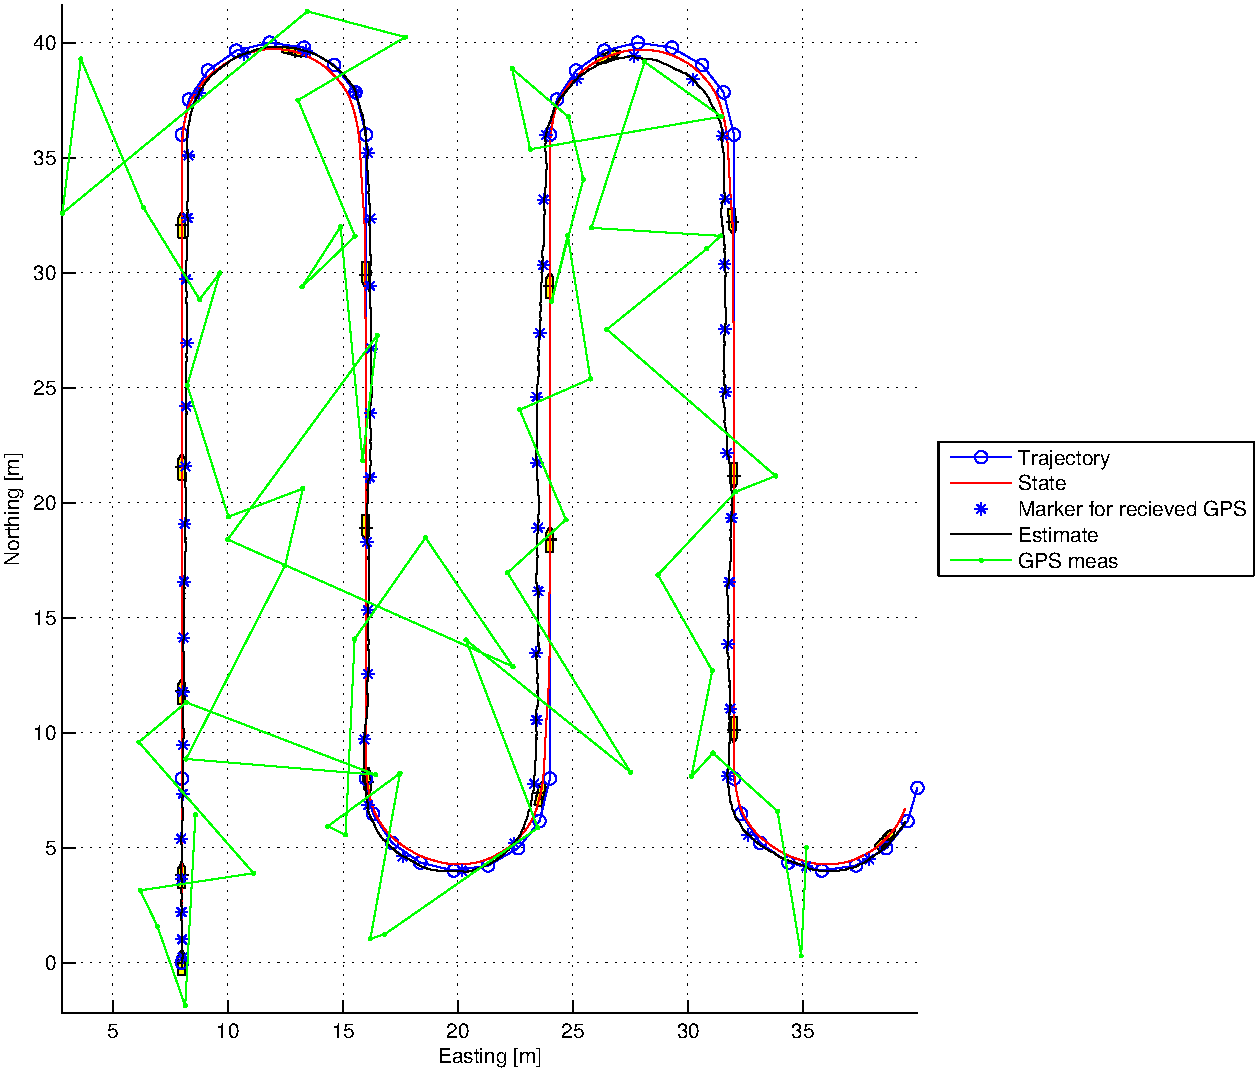
\includegraphics[width=0.48\textwidth]{../code/matlab/q0,0001}
% \caption{Simulation}
% \end{center}
% \end{wrapfigure}

%As for now shows the simulation that the model of the AAUSHIP are able
%to follow a predetermined trajectory with a mean error of 32cm and a
%maximum error of 87cm. This is within the accepted limit when looking
%at the area of interest. When then AAUSHIPs needs to sail in
%formation, and cover rather large areas, then is the accuracy not very
%important, at least not such small derivations.

The result of the project is expected to be a complete
survey of a bounded area from the use case given by the Port of
Aalborg. This is used in a comparison with data measured from the Port
of Aalborg to verify the AAUSHIP survey system, as this will end up
being. This map needs to be measured by two or three autonomous
vessels that sails in a predetermined formation that has not yet been
decided. The formation approach still needs to be chosen. Work on
testing three different candidate strategies is the goal. 
 
\paragraph{Conclusion}
For now the first aim is reached with a model of the AAUSHIP that can
track the given trajectory, implementation of the whole ship is close
to done, it just needs testing. Moving on the focus is to determine
the control paradigms within formation control that fits with our
use case and implement this on AAUSHIP and the rest of the fleet.

%As the complete
%conclusion should the tests be performed in the same location of
%interest as the data have been taken by the Port of Aalborg. The
%conclusion should by that time be that the fleet can do it as good as
%the manual scanning performed by The Port of Aalborg.



\end{document}

%Here's a suggestion as to what an extended abstract should contain:
%
%    Background - A little history about who's done what and how your work fits in with it.
%    Aim - What you're trying to tell the audience that they don't already know (e.g. Your story.)
%    Method - Why the audience should believe that the results you've got aren't made up or flawed
%    Results - Evidence that you've come up with that confirms your story
%    Conclusion - Recap of your story and its implications
%    Limitations - Why someone might doubt your story and what you've done to get rid of as much doubt as possible.
%
%What if I'm presenting a review of my progress to date and I have no original research?
%Method = literature survey.
%Results = what you've read.
